\documentclass{ametsoc}
\usepackage[]{graphicx}
\usepackage{alltt}
\usepackage{siunitx}
%
%==============================================================================
\journal{jcli}

%
%==============================================================================
\bibpunct{(}{)}{;}{a}{}{,}

\title{Effects of Natural Variability of Seawater Temperature, Time Series Length, Decadal Trend, and Instrument Precision on the Ability to Detect Temperature Trends}

\authors{Robert Schlegel\correspondingauthor{Robert Schlegel, Department of Biodiversity and Conservation Biology, University of the Western Cape, Bellville, Republic of South Africa.}
 and Albertus Smit}

\affiliation{Department of Biodiversity and Conservation Biology, University of the Western Cape, Bellville, Republic of South Africa}

\email{wiederweiter@gmail.com}

%
%==============================================================================
\abstract{In South Africa 129 \emph{in situ} temperature time series of 1 to 43 years are used for investigations of the thermal characteristics of coastal seawater. They are comprised of temperature recordings at precisions ranging from \SIrange{0.5}{0.001}{\degreeCelsius} and collected with handheld thermometers or underwater temperature recorders (UTRs). Using the naturally occurring range of seasonal signals, variability and temperature trends for 84 of these time series, the length, decadal trend, and data precision of each time series were systematically varied before fitting generalized least squares (GLS) models to study the effect these variables had on trend detection. We determined that low instrument precision has less effect on the ability of a model to detect trends within a time series than does the length, variance or the decadal trend itself, with length contributing the most to trend detection. We found that time series at least 20 years in length may be used tentatively for climate change research, but that time series >30 years in length are preferable. The implication is that long-running thermometer time series in this dataset, and others around the world, are more useful for decadal scale climate change studies than the shorter, more precise UTR time series.}

% AJS: At the same length, which is most useful: thermometer or UTR recordings?
% RWS: Given everything I've learned of instrument precision and the results of these analyses, I would say they are the same. I was going to say so in the abstract but decided against it. I need to perform an investigation into this by comparing closeness of fit to DT_model and DT with varying length against the different types. I think thermo's may actually be better....

%==============================================================================
\begin{document}

\maketitle

\section{Introduction}
The roughly ~3,000 km of South Africa's coastline is bordered by the Benguela and Agulhas currents \citep[e.g.][]{Roberts2005,Hutchings2009}, which, in combination with other nearshore processes, affect the country's marine coastal ecosystems \citep{Santos2012a}. A thorough understanding of these coastal processes is provided by several physical variables, of which temperature is one of the main determinants \citep[e.g.][]{Blanchette2008, Tittensor2010, Couce2012}. In order to ensure a true representation of organisms' biological thermal limits, nearshore temperatures must be accurately recorded and monitored. Whereas some sources warn of the pitfalls in doing so \emph{RWS: Add references here showing which sources say using SST for the coast is inappropriate}, a widespread approach in coastal ecological research is to use satellite and/or model-generated temperature data as representation of the sea surface temperature (SST) along coastlines \citep[e.g.][]{Blanchette2008, Broitman2008a, Tyberghein2012}. However, a study by \citet{Smit2013} showed that SST data may have a warm bias as large as \SI{6}{\degreeCelsius} when compared to coastal \emph{in situ} data. It is for this reason that the authors strongly recommended the use of \emph{in situ} data to support research conducted within 400 m from the shoreline.

Even though records of \emph{in situ} coastal seawater temperature exist, the reliability of many of these datasets that could be used in place of the remotely-sensed SST data remains to be verified. Users of SST data benefit from it being refined through a number of well documented validation and quality control processes \citep[e.g.][]{Reynolds1994, Brown1999, Martin2012}, whereas the standards and methods with which local \emph{in situ} data from a single dataset are collected and refined may differ greatly. For example, there are currently seven organizations and/or governmental departments (hereafter referred to as bodies) contributing coastal seawater temperature data to the South African Coastal Temperature Network (SACTN). These bodies use different methods and instruments to collect their data as no national standard has been set. One consequence of this methodological disparity is that two thirds of the data were sampled with hand-held thermometers that are manually recorded at a data precision of \SI{0.5}{\degreeCelsius}, as opposed to the current generation of Underwater Temperature Recorders (UTRs) with an instrument precision of up to \SI{0.001}{\degreeCelsius}. If these \emph{in situ} data are to be used together \emph{in lieu} of the satellite-based SST data, it is important that the characteristics of the contributing data sources are understood in terms of their ability to yield useful, reliable and accurate long-term measurements for use in climate change studies.

This prompted us to examine the 129 \emph{in situ} time series that comprise the SACTN, whose locations and instrument types may be seen in Figure \ref{figure01}. The ranges of data precision and statistical characteristics found within this dataset were used to guide a series of hypotheses driven analyses into the suitability of the time series to yield statistically significant assessments of decadal temperature change. The length, decadal trend and data precision of each time series were adjusted in a systematic manner, and forms the core of our analyses. Our aim was to assess the effect that each of these variables has on the ability of a model to detect a decadal trend within a time series. The effect data gaps may have on the fitting of models was also investigated as many of the time series used here have missing months of data scattered throughout, which is unavoidable for a 20+ year time series that is sampled by hand by a single technician at each site.

The study provides a better understanding of some of the determinants of a time series that are influential in the detection success of decadal trends in coastal ocean temperature time series.

\emph{RWS - This sentence doesn't fit well with how I reworded the paragraphs: "It is for this reason that data precision was one of the primary foci in these analyses."}

\emph{AJS - what about this? Did we study this systematically? Must it be removed? "The effect data gaps may have was investigated as many of the time series used here have missing months of data scattered throughout, which is unavoidable for a 20+ year time series that is sampled by hand by a single technician at each site."}
\emph{RWS - The data gaps were not studied systematically, but rather a correlation is drawn between p_trend and NA\%}

\section{Methods}

\subsection{Data Sources}
Our study lies within the political borders of South Africa's coastline. The location of each point of collection may be found in Figure \ref{figure01}. Of the 129 time series used, 43 are recorded with UTRs and the other 86 with hand-held mercury thermometers. The oldest currently running time series began on January 1st, 1972; there are 11 total time series that started in the 70s, 53 more started in the 80s, 34 began in the 90s, 18 in the 00s and 13 in the current decade.

The data are collected using two different methods and a variety of different instruments. Hand-held mercury thermometers (which are being phased out in favor of alcohol thermometers or electronic instruments) are used in some instances from the shoreline, and represent seawater temperatures at the surface. At other places, predominantly along the country's east coast, data are collected with glass thermometers from a small boat at the location of shark nets along the coast \citep{Cliff1988}. Data at other localities are collected using delayed-mode instruments that are permanently moored shallower than 10 m, but generally very close to the surface below the low-water spring tide level.

Over the last 40+ years the electronic instruments used have changed and improved. The previous standard was the Onset Hobo UTR with a thermal precision of \SI{0.01}{\degreeCelsius}. The meta-data pertaining to these older temperature records and to those that came before, such as the instrumentation used and the motivation behind the levels of precision at which the data were recorded, have over time been lost, highlighting the issues of staff rotation in government departments and the importance of implementing meta-data standards at a very early stage in any monitoring programme. The new standard currently being phased in is the Starmon Mini UTR. These devices have a maximum thermal precision of \SI[separate-uncertainty = true, multi-part-units = repeat]{0.001(25)}{\degreeCelsius} (http://www.star-oddi.com/). Of the 43 UTR time series in this dataset, 30 were recorded at a precision of \SI{0.001}{\degreeCelsius} for their entirety, five UTR time series include older data that were recorded at a precision of \SI{0.01}{\degreeCelsius} or \SI{0.1}{\degreeCelsius} and so have been rounded down to match this level of precision. Eight additional UTR time series have older data that were recorded at a precision of \SI{0.1}{\degreeCelsius}. UTR time series recorded entirely at a precision of \SI{0.001}{\degreeCelsius} are grouped in the `new' subgroup of time series and those with data recorded at lower precisions are grouped in the `old' subgroup. Time series recorded with handheld thermometers have been grouped in the `thermo' subgroup. We provide no information about the accuracy of the temperature recordings.

\emph{AJS - Referring to the above paragraph: Do we still have to refer to the 'thermo,' 'new' and 'old' subgroups?}
\emph{RWS - I have a cunning plan to show the differences in models fitted to these different instrument types so it is worth still referring to them here.}

The thermometer data are recorded manually and saved in an aggregated location at the head offices of the collecting bodies. UTRs are installed and maintained by divers and data are retrieved at least once annually. These data are digital and are downloaded to a hard drive at the respective head offices of the collecting bodies.

\subsection{Data Management}
Each of the seven bodies contributing data to this study have their own method of data formatting. Steps are being taken towards a national standard as we move towards replacing all the thermometer recordings with UTR devices; however, as of the writing of this article, one does not yet exist. Data from each organization were formatted to a project-wide comma-separated values (CSV) format with consistent column headers before any statistical analyses were performed. This allowed for the same methodology to be used across the entire dataset, ensuring consistent analysis. Before analysing the data they were scanned for any values above \SI{35}{\degreeCelsius} or below \SI{0}{\degreeCelsius}. These data points were changed to \texttt{NA}, meaning `not available', before including them in the SACTN dataset.

All analyses and data management performed in this paper were conducted with R version 3.3.1 (2016-06-21) \citep{R}. The script and data used to conduct the analyses and create the tables and figures in this paper may be found at https://github.com/schrob040/Trend_Analysis.

Any time series with a temporal precision greater than one day were meaned into daily values before being aggregated into the SACTN. A series of additional checks were then performed (e.g. removing long stretches in the time series without associated temperature recordings), missing values interpolated when it was deemed safe to do so and time series shorter than five calendar years or collected at depths greater than 10 m were removed. At the time of this analysis, this daily dataset consisted of 84 time series, consisting of 797,736 days of data; these data were then binned further to the 26,209 monthly temperature values available for use in this study.

%The 129 time series were then visually inspected for any obvious errors, gaps or irregularities. Several consecutive years of missing data were found within eight time series. Of these, three were discarded outright and 207 total months without temperature recordings were removed from the other five time series, either from the leading or trailing side of the time series. Of the remaining 126 time series, five more were removed as they were collected at depths greater than 10 m. A minimum length of five years was then imposed, removing a further 33 time series. Finally, four more time series missing more than 15\% of their monthly values were removed, making for a total of 84 time series and 25,636 complete months of data.

\emph{AJS - I am not so sure the above para is needed anymore; since we are not using the data for actual trend detection we do not need to be too anal about the quality of the time series. Also, I suppose considering that we are not using the coastal classification scheme anymore that it is not necessary to fuss too much about the >10 m time series... I have added a small blurb in the preceding para to quickly summarise all of this stuff.}
\emph(RWS - I think the depth limit is still worth imposing as the deeper time series likely have different seasonal and long term signals than the shallower time series. Also, I'd rather not run the models again... I added in why time series were removed as it is necessary to know why the dataset was trimmed down from 129 to 84 time series for the sake of continuity in the paper.}

%To address the effect outliers may have on the summaries of the ranges for values presented in this paper, the 5th and 95th percentiles are given rather than the minimum and maximum values. \emph{RWS - Does this even need to be validated here? Can't it just be mentioned in the caption for the tables it applies to?}

\emph{I don't think this (above) is relevant anymore... although the assumption of normality of data is still valid and needs to be demonstrated; a series of box and whisker plots summarising the data (median, 25th and 75th, 5th and 95th percentiles) will be useful! I'll make one later this evening.-Sorted}.

\subsection{Systematic Analysis of Time Series}
We used the 84 time series simply for their variance properties (comprised of seasonal, interannual, decadal and ‘noise’ components), which reflect that of the thermal environment naturally present along the ~3,000 km of South African coastline. Unknown linear trends that may have been present in each time series were removed prior to the ensuing analyses by applying an ordinary least squares regression and keeping the detrended residuals. In doing so we avoided the need to simulate a series of synthetic time series, whose variance components may not have been fully representative of that naturally present in coastal waters. Furthermore, these detrended time series represent a range of time scales, from 5 to 43 years in duration. \emph{We could add a Table that summarises all of these properties, maybe…?}. \emph{RWS - I'll look into how best to make/ present these tables.}

It is important to note that the linear interpolation used to fill the \texttt{NAs} in the time series may have artificially increased the goodness of fit of the detected trend. A simple linear regression between the goodness of fit (\emph{R}\textsuperscript{2}) and proportion of missing values (hereafter referred to as NA\%) for all time series was applied to better understand this potential relationship. \emph{RWS: This was done and drama ensued. Needs to be altered to adressed how that all played out. Perhaps it should be discussed in the results.}

We acknowledge that the selection of the appropriate model can greatly influence the ability to detect trends \citet{Franzke2012}. Two broad approaches are widely used in climate change research (cite: IPCC, 2013). The first group of models estimates linear trends, and although linearity may not reflect reality (\emph{i.e.} trends are very frequently non-linear), these models do provide the convenience of producing an easy to understand decadal trend (\si{\degreeCelsius}~dec$^{-1}$) (insert refs here). The other group accommodates non-linear trajectories of temperature through time by the use of higher-degree polynomial terms or non-parametric smoothing splines, but the inconvenience comes from not being able to easily compare models among sites (insert refs here). Both groups of models can accommodate serially correlated error structures, which is often the cause for much criticism due to their effect on the uncertainty of the trend estimates (insert refs here). For example, Generalized Least Squares (GLS; yielding estimates of linear trends) and Generalized Additive Mixed Models (GAMM; non-linear fitting) can both capture various degrees of serial autocorrelation (insert refs here). Although our exploratory analyses assessed two parameterizations with each of the model groups, we opted to proceed here with GLS equipped with a second-order autoregressive AR(2) correlation structure (cite: Wood, 2006), which is similar to that used by the IPCC (IPCC, 2013). In this way we could assess how various properties of the detrended data sets would affect the model’s ability to detect trends --- in other words, by comparing the estimates of the trends themselves.

To each of the 84 detrended time series we artificially added linear decadal trends (0.00, 0.05, 0.10, 0.15 and 0.20 \si{\degreeCelsius}~dec$^{-1}$). In other words, we now had time series that captured the natural thermal variabilities around the coast, but with their decadal trends known \emph{a priori}. The range of decadal trends was selected based on the global average of \emph{RWS: Insert correct value here.} \SI{xx}{\degreeCelsius} (cite: IPCC, 2013). Furthermore, in order to replicate the instrumental precision of the instruments used to collect these time series, we rounded each of these (84 time series \texttimes{} 5 decadal trends) to four levels of precision: \SI{0.5}{\degreeCelsius}, \SI{0.1}{\degreeCelsius}, \SI{0.01}{\degreeCelsius} and \SI{0.001}{\degreeCelsius}. Consequently, we had a pool of 1,680 time series on which to fit our GLS model.

This approach allowed us to study the effect that the relevant variables (length, natural variability, added slope and level of measurement precision) within each time series have on the ability of the GLS to faithfully detect the decadal thermal trend, which was known \emph{a priori}. The primary results of interest in these analyses were the significance (\emph{p}-value) of the model fit, the magnitude of the decadal trend determined by the GLS model as well as the error associated with the trend estimate. \emph{AJS – talking about the length… are we keeping this? If so, I’ll edit the next bit of text and make more graphs to show this effect… “To determine this, each time series was first shortened to a minimum length of 5 years, starting in January so that the timing of the seasonal signal for each time series would be equitable. After fitting the GLS model to the all 84 of the shortened time series, the next year of data for each time series was added and the models fitted again. This process was repeated for the full length of each time series. For example, if a time series consisted of 12 full years of data (144 months), it would have 8 models fitted to it. A 40 year (480 month) time series would have 36 models fitted to it. This required 36,220 GLS models to be fitted to the "flat" time series.”}

\emph{RWS - As length has by far the greatest impact on the faithful detection of DT, I think we should definitely keep this. Also, without this "growth" of lengths, there is almost no real replication in the experimental design.}

\emph{RWS - I've had another think over my answer above and perhaps we can do without growing the model. I still want to show the realtionship length has with the other variables, but that can probably be done without growing the time series....}

\emph{AJS – see the refs below. I would send you the IPCC thing, but it is too big. If you have decent internet access at home you can download it. There is also a supplement, which I have emailed you (see page 2SM-10). Anyway, the main document is the important one, because there (on page 179) you will find various references that you can use to insert into the portions above where I indicated references are needed.}

References
Wood, S.N. (2006) Generalized Additive Models: an introduction with R, CRC
IPCC, 2013: Climate Change 2013: The Physical Science Basis. Contribution of Working Group I to the Fifth Assessment Report of the Intergovernmental Panel on Climate Change [Stocker, T.F., D. Qin, G.-K. Plattner, M. Tignor, S.K. Allen, J. Boschung, A. Nauels, Y. Xia, V. Bex and P.M. Midgley (eds.)]. Cambridge University Press, Cambridge, United Kingdom and New York, NY, USA, 1535 pp.



\section{Results}

\emph{RWS: These results have been removed as the classification is no longer being performed.}
%\subsection{Coastal Classification}
%The coastal classification resulted in three groups, each reflecting distinct thermal properties. The August and February SD values have a larger effect on the west and south coast groups than the August and February median values, which largely influence the grouping of the east coast time series. The range values have the most prevalent effect on the south coast time series, as would be expected due to the larger inter-annual variation occurring there. We see in Figure \ref{figure02} that some peculiarities exist in the coastal allocation of a few time series; explanations for these geographical outliers involve nuances of the physical oceanographic forcings operating at these sites, and will not be further discussed here.

\emph{RWS: This subsection has been removed and some of the text has been moved to the new subsection.}
%\subsection{Time Series Analysis}
%Table \ref{range-table} shows the range in relevant variables for the different coastal groupings and instrument types. The results from the time series analysis on all of the thermal data may be seen in Tables A1--3. The range of $\Delta T$ values detected in the time series analysis was surprisingly large with the maximum and minimum values for time series 10+ years in length ranging from \SIrange{-1.1}{1.4}{\degreeCelsius}~dec$^{-1}$. The mean and median values of the $\Delta T$ for 10+ year time series were \SI{0.17}{\degreeCelsius}~dec$^{-1}$ and \SI{0.10}{\degreeCelsius}~dec$^{-1}$. The aforementioned range of $\Delta T$ values for 10+ year time series is attributable to the thermometer data, with the range of $\Delta T$ for old UTR data smaller at \SIrange{-0.2}{1.2}{\degreeCelsius}~dec$^{-1}$. There is only one new UTR time series that is both 10+ years in length and shallower than 10 m, the $\Delta T$ for this time series is \SI{-0.174}{\degreeCelsius}~dec$^{-1}$.

%The \emph{R}\textsuperscript{2} values, representing the linearity of the trend, for 10+ year time series ranged from 0.00 to 0.58, with a mean and median of 0.12 and 0.08. The thermometer data were again responsible for this maximum range in values with the range for the old UTR data at 0.00 to 0.48 and the one qualifying new UTR time series had a \emph{R}\textsuperscript{2} value of 0.02.

%The \emph{R}\textsuperscript{2} values of some time series were much greater than others. This is in part due to the short duration of these time series, allowing for less time in which competing signals may weaken the overall linearity of the trend in the time series. However, we have just shown that the new UTR time series that is 10+ years in length has a smaller \emph{R}\textsuperscript{2} value than the majority of the time series in this dataset. To further investigate the effect the length of a time series has on linearity, the relationship between the \emph{R}\textsuperscript{2} and length of each time series was fitted to a simple linear model. It was found that the positive relationship was significant (\emph{p}\num{< 0.001}) with an \emph{R}\textsuperscript{2} of 0.11.

%As one can see in Table \ref{range-table}, the east coast subgroup may have time series of a longer median length than the other two coastal subgroups; however, the difference in median lengths between UTR data and thermometer data is larger. We also see that while the maximum proportion of missing values (hereafter referred to as NA\%) for the thermometer data is greater than either UTR types, the median NA\% for the thermometer data is less than both UTR types. Similarly, the east coast time series have fewer missing data than those from the west and south coasts, which are comparable. The east and west coasts have similar SD values, whereas the south coast has much more variance. The thermometer data have more variance than the old UTR data, which in turn have more variance than the new UTR data.

%A simple linear regression between \emph{R}\textsuperscript{2} and NA\% for all time series reveals the goodness of fit for this relationship to be 0.01 with a \emph{p}-value of 0.205. When the time series with large gaps are screened and the same linear model is applied to the relationship between NA\% and \emph{R}\textsuperscript{2} for time series with 10\% NA or less the goodness of fit drops to 0.00 and the \emph{p}-value increases to 0.473.

% The findings of the analysis of time series shorter than 10 years in duration are covered in the Discussion.

\emph{RWS: This subsection has been removed as the results are no longer relevant to the aims.}
%\subsection{Power Analysis}
%Figure \ref{figure03} shows the 25th, 50th (median), and 75th percentile for the power analysis for each subgroup. The 5th and 95th percentiles have been excluded from this boxplot because several very low \emph{r} values drive the 95th percentile to extraordinarily large values and the 5th percentile has been removed for balance. The east coast subgroup has the largest range of required months to obtain a power of 0.80 at 43 to 324 and the largest range for power 0.90 at 56 to 432 months. This subgroup also has the largest required median for power 0.80 and 0.90 at 127 and 169 months respectively. The new UTR time series have the smallest range of required months for power 0.80 at 21 to 35 months and a range for power 0.90 from 28 to 45 months. This subgroup also has the shortest required median number of months for power 0.80 and 0.90 at 27 and 35, respectively.

\emph{RWS - The first 5 paras are from the "Time Series Analysis" results subsection.}
\subsection{Systematic Analysis of Time Series}

% A broad overview of all the results can include:
% * the significance (\emph{p}-value) of the model fit
% * the magnitude of the decadal trend determined by the GLS model
% * the error associated with the trend estimate
% * the effect missing% of time series has on the other variables
%
% Then go to the primary research questions are these:
% * the effect of length on the other variables (i.e. 1. the model trend converging to the actual trend [all_plt2.pdf]; 2. the ratio of the actual trend to the model trend and SE of fit [all_plt6.pdf]; 3. the effect of initial SD and length on the SE of the model trend [all_plt7.pdf])
% * the effect of different decadal trends on the other variables (these are incorporated into all_plt2.pdf, all_plt6.pdf and all_plt7.pdf).
% * the effect of different precisions on the other variables [correlations_new.pdf] and the correlation and RMSE values.
% * the effect of different instrument types, controlling for all other dependent and independent variables

% A broad overview of all the results
The range of relevant variables may be found in Table \ref{table01}.

\subsection{Magnitude of decadal trend determined by GLS}
As would be expected, the larger the decadal trend (DT) added to the detrended data was, the larger the trend detected by the GLS model became. The accuracy of the model however changed little as DT was increased. Rather, the natural variance found within the detrended time series had a larger effect on the modelled trend.

\subsection{Significance (\emph{p}-value) of the model fit}
The signifance (\emph{p}) of the trends detected by the GLS models ranged from XX to XX, with a mean of XX. The thermometer data were again responsible for this maximum range in values with the range for the old UTR data at XX to XX and the new UTR time series had  \emph{p} values of XX to XX.

\subsection{Error associated with trend estimate}
Figure \ref{figure03} shows that the SD of a time series has a large effect on the significance of that fit. Of the 105 time series used in this step of the analysis, 84 were significant when the SD of the noise component of the time series was \SI{0.2}{\degreeCelsius}. Halfway through the analysis when the SD was raised to \SI{0.7}{\degreeCelsius}, 67 time series still remained significant at $\emph{p} \leq 0.05$. At the final step when SD was raised to \SI{1.3}{\degreeCelsius} only 43 time series remained significant at $\emph{p} \leq 0.05$. The increase in \emph{p} values as SD was raised from \SIrange{0.2}{1.3}{\degreeCelsius} was greatest for the old UTR data at 0.147 (from 0.002 to 0.149) and smallest for the west coast subgroup at 0.052 (from 0.000 to 0.052). The effect increases in SD had on \emph{R}\textsuperscript{2} values was not negligible with the new UTR time series most affected, showing a decrease in median \emph{R}\textsuperscript{2} values by 0.08 (from 0.33 to 0.25). The data from the east coast subgroup showed the smallest decrease in \emph{R}\textsuperscript{2} at 0.01 (from 0.08 to 0.07). Whereas the median \emph{R}\textsuperscript{2} values for the subgroups show little change as SD is increased, the 95th percentiles for these data (the top of the grey ribbon) show large rates of decrease with the east coast subgroup having the greatest decrease of any of the subgroups with a range of 0.32 (from 0.77 to 0.46). With the exception of the new UTR data, the other subgroups of data had similar ranges in decrease for the 5th and 95th percentiles as SD was increased with \emph{R}\textsuperscript{2} values of 0.45 to 0.50 when SD was \SI{1.3}{\degreeCelsius}.

\subheading{Effect of \% missing values on trends estimation}
We also see that while the maximum proportion of missing values (hereafter referred to as NA\%) for the thermometer data is greater than either UTR types, the median NA\% for the thermometer data is less than both UTR types. The thermometer data have more variance than the old UTR data, which in turn have more variance than the new UTR data.

A correlation between the significance of the trends detected by the GLS model and the NA\% for all time series reveals the goodness of fit for this relationship to be 0.XX with a \emph{p}-value of 0.XX. Further analysis however proved this relationship to not be so clear. WHen values When the same linear model is applied to the relationship between NA\% and \emph{R}\textsuperscript{2} for time series with 10\% NA or less the goodness of fit drops to 0.00 and the \emph{p}-value increases to 0.473. The rate of decrease in \emph{R}\textsuperscript{2} as NA\% decreases is XX, meaning that an NA\% of XX could significantly affect the model output.

Much of the range seen in the results from the GLS models can be explained in by their relation to the independent variables. Namely, the length of the time series, the decadal trend added and the precision of the data.

\subsection{Effect of time series length on trend estimation}
(i.e. 1. the model trend converging to the actual trend [all_plt2.pdf]; 2. the ratio of the actual trend to the model trend and SE of fit [all_plt6.pdf]; 3. the effect of initial SD and length on the SE of the model trend [all_plt7.pdf])
As one can see in Table \ref{table01}, there is a large difference in mean lengths between the new and old UTR data and the thermometer data. It is therefore important to measure the effect length has on the other results given above so as to not cause undue bias towards the usefulness of the much longer thermometer data.

To determine the effect length of a time series had on the statistics seen in Table \ref{table01}, the relationship between these values and length of each time series was fitted to a simple linear model. It was found that the positive relationship was significant (\emph{p}\num{< 0.XX}) with an \emph{R}\textsuperscript{2} of 0.XX. \emph{RWS: Repeat for each statistic.} These relationships are shown in Figure \ref{figure02} etc.

\subsection{Effect of initial SD on trend estimate}
Blurb goes here...

\subsection{Effect of decadal trend steepness on trend estimation}
(these are incorporated into all_plt2.pdf, all_plt6.pdf and all_plt7.pdf).
Increasing the size of the DT added to the detrended time series had a large effect on the models ability to accurately detect a signal. This ranged from XX when 0.00\si{\degreeCelsius}~dec$^{-1}$ was added and XX when 0.20\si{\degreeCelsius}~dec$^{-1}$ was added.

\subsection{Effect of measurement precision on trend estimation}
[correlations_new.pdf] and the correlation and RMSE values.
The effect of decreasing data precision from \SI{0.001}{\degreeCelsius} to \SI{0.5}{\degreeCelsius} had almost no effect on the 5th, 50th (median) and 95th percentiles. There is an increase in the median \emph{R}\textsuperscript{2} value for the new UTR data of 0.01 (from 0.25 to 0.26) when the data are rounded from \SIrange{0.001}{0.5}{\degreeCelsius}. The same rounding has no effect on the range of the 95th percentile but does increase the 5th percentile \emph{R}\textsuperscript{2} value by 0.01 (from 0.09 to 0.10). Rounding the data to \SI{1.0}{\degreeCelsius} has a much larger effect. The median \emph{R}\textsuperscript{2} value for the new UTR data increase by 0.04 (from 0.25 to 0.29), the 95th percentile increase by 0.03 (from 0.70 to 0.73) and the 5th percentile does not change. Whereas decreasing the data precision of the new UTR time series had a measurable effect on the \emph{R}\textsuperscript{2} value of the linear models fitted to them, it had no effect on the \emph{p} value of those linear models. All trends in the new UTR time series remained significant at $\emph{p} \leq 0.001$ regardless of the level of data precision.

\subsection{Effect instrument type on trend detection}
...on controlling for all other dependent and independent variables
When questioning which types of data produce larger ranges of $\Delta T$ values (with larger rates of linearity) from time series under 10 years, we see that the range of $\Delta T$ (\emph{R}\textsuperscript{2}) values for thermometer data at \SI{-1.9}{\degreeCelsius}~dec$^{-1}$ (0.28) to \SI{3.5}{\degreeCelsius}~dec$^{-1}$ (0.69) is similar to those for the old UTR data with a range from \SI{-5.0}{\degreeCelsius}~dec$^{-1}$ (0.52) to \SI{0.4}{\degreeCelsius}~dec$^{-1}$ (0.7); however, the new UTR data have by far the largest range from \SI{-7.233}{\degreeCelsius}~dec$^{-1}$ (0.81) to \SI{2.576}{\degreeCelsius}~dec$^{-1}$ (0.29). These very large $\Delta T$ and \emph{R}\textsuperscript{2} values serve as a strong example of the necessity for longer time series.




\section{Discussion}

\emph{RWS: This subsection has been removed and some of the text has been moved to the new subsection.}
%\subsection{Time Series Analysis}
%The time series analysis was applies to time series as short as 3 years at the risk of producing more erratic values in order to analyse as many of the time series in the dataset as possible. The smaller \emph{n} for these time series allows any short-term phenomena to have a larger impact on the detected decadal change than in the longer time series, which may give the illusion that some of the shorter time series are showing very significant results in terms of decadal change. For example, the largest $\Delta T$ (\emph{R}\textsuperscript{2}) values at either end of the spectrum for time series at or under 10 years in length are \SI{3.5}{\degreeCelsius}~dec$^{-1}$ (0.69) and \SI{-7.233}{\degreeCelsius}~dec$^{-1}$ (0.81). The highest \emph{R}\textsuperscript{2} value for any time series at or under 10 years is 0.81. These extrapolated decadal trend values could not to be sustained over a long period as almost any point in the ocean would freeze over in only 40 years at \SI{-7.233}{\degreeCelsius}~dec$^{-1}$! Not all short time series have large $\Delta T$ (\emph{R}\textsuperscript{2}) values; indeed, the lowest $\Delta T$ (\emph{R}\textsuperscript{2}) value for time series under 10 years is \SI{0.0}{\degreeCelsius}~dec$^{-1}$ (0.00). The mean and median values for $\Delta T$ from time series under 10 years are \SI{0.08}{\degreeCelsius}~dec$^{-1}$ and \SI{0.25}{\degreeCelsius}~dec$^{-1}$.

%\emph{AJS: Above the trend data are reported at two levels of precision... I think you need a statement somewhere near the start of the section here, or in the Results section, saying that the more precise reporting is for the UTR data while the lower precision trends were only provided for the other data. Or something like that... It looks weird when there is three decimal places some times, and only one other times.}

%When questioning which types of data produce larger ranges of $\Delta T$ values (with larger rates of linearity) from time series under 10 years, we see that the range of $\Delta T$ (\emph{R}\textsuperscript{2}) values for thermometer data at \SI{-1.9}{\degreeCelsius}~dec$^{-1}$ (0.28) to \SI{3.5}{\degreeCelsius}~dec$^{-1}$ (0.69) is similar to those for the old UTR data with a range from \SI{-5.0}{\degreeCelsius}~dec$^{-1}$ (0.52) to \SI{0.4}{\degreeCelsius}~dec$^{-1}$ (0.7); however, the new UTR data have by far the largest range from \SI{-7.233}{\degreeCelsius}~dec$^{-1}$ (0.81) to \SI{2.576}{\degreeCelsius}~dec$^{-1}$ (0.29). These very large $\Delta T$ and \emph{R}\textsuperscript{2} values serve as a strong example of the necessity for longer time series.

%That there is no significant relationship between the goodness of fit (\emph{R}\textsuperscript{2}) and NA\% of the time series in this study is an encouraging result and suggests that linear interpolation is an acceptable method of filling in missing data in a time series analysis, but should be avoided where possible.

\emph{AJS: Is the above small para not an exact contradiction to line 109 in the .tex file?}
\emph{RWS: The line numbers have been changed but if I am reading the correct line, it is saying that there is a significant relationship between length and goodness of fit. Not NA\% and goodness of fit as here.}

\emph{RWS: This subsection has been removed as the discussion is no longer relevant to the aims.}
%\subsection{Power Analysis}
%The presence of very small correlation (\emph{r}-values) for most subgroups led to the power analyses showing a massive range of \emph{n} values required to reach a power of 0.80 or 0.90. The largest \emph{n} projected is 86,833 months. This means that the correlation between temperature and time in some time series was so small that one would required several thousand years of data in order to develop confidence in the detected trend. As this would prevent a meaningful display of the results relevant to this study, only values within the 25th to 75th percentiles were used, as seen in Figure \ref{figure03}.

%The boxplots in Figure \ref{figure03} are skewed to the left because a very large \emph{r}-value can only reduce the \emph{n} required for the desired power so much before approaching 0, whereas a very small \emph{r}-value can extend the required \emph{n} to a much greater extent. There are also large differences in the 75th percentiles for the different subgroups. The required \emph{n} for the new UTR data is noticeably lower than for the other groups, perhaps leading to the erroneous conclusion that the short median length of these time series (68 months) may be causing the strong correlations. However, when we relate \emph{r} to length of each time series using a simple linear model the resultant \emph{R}\textsuperscript{2} and \emph{p} are 0.00 and 0.241, meaning that there is no significant relationship between the length of a time series and how linear its decadal trend is. The stronger results for the west coast, south coast and new UTR subgroups may be attributed to their smaller sample sizes, as noted in Figure \ref{figure03}. The majority of the \emph{n} values in the west coast, south coast and new UTR subgroups are simply much smaller than the other groups, and this is simply by chance, as evinced by the much larger 75th percentile for the old UTR subgroup, which also has a small sample size. If these subgroups were to have more time series added their mean and 75th percentile values would increase to look more like the total average as seen in the all subgroup.

\emph{RWS: This subsection contains three paragraphs from the "Time Series Analysis" discussion subsection.}
\emph{RWS: None of this text has been edited. I must still do so.}
\subsection{Systematic Analysis of Time Series}

% The primary research questions to duiscuss:
% * the effect of variance on the other variables
% * the effect NA% has on the other variables
% * the effect of length on the other variables (i.e. 1. the model trend converging to the actual trend [all_plt2.pdf]; 2. the ratio of the actual trend to the model trend and SE of fit [all_plt6.pdf]; 3. the effect of initial SD and length on the SE of the model trend [all_plt7.pdf])
% * the effect of different decadal trends on the other variables (these are incorporated into all_plt2.pdf, all_plt6.pdf and all_plt7.pdf).
% * the effect of different precisions on the other variables [correlations_new.pdf] and the correlation and RMSE values.
% * the effect of different instrument types, controlling for all other dependent and independent variables

% * the effect of variance on the other variables
When the largest SD of \SI{1.3}{\degreeCelsius} was applied to the time series in these data it increased the \emph{p}-value of the decadal trends detected above 0.05. This implies that if one is sampling seawater temperature in a highly variable area, collecting an additional decade of data may not allow one to establish a significant trend. Consequently, one must take into account the natural variability of the seawater temperatures in a study area when determining how many months of data may be required before climate change studies become feasible.

% * the effect NA% has on the other variables
That there is a significant relationship between the significance of the detected trend and the NA\% of time series in this study. Interestingly, the amount of missing data in a time series affects the behavior of the GLS model differently. Furthermore, if the missing data are linearly interpolated this effect becomes even more pronounced. This means that linear interpolation is not an acceptable method of filling in missing data in a time series analysis and should be avoided where possible.

% * the effect of length on the other variables (i.e. 1. the model trend converging to the actual trend [all_plt2.pdf]; 2. the ratio of the actual trend to the model trend and SE of fit [all_plt6.pdf]; 3. the effect of initial SD and length on the SE of the model trend [all_plt7.pdf])
\emph{RWS: This para must be altered to discuss how short time series affect the models ability to detect the given DT.}
The time series analysis was applies to time series as short as 5 years at the risk of producing more erratic values in order to analyse as many of the time series in the dataset as possible. The smaller \emph{n} for these time series allows any short-term phenomena to have a larger impact on the detected decadal change than in the longer time series, which may give the illusion that some of the shorter time series are showing very significant results in terms of decadal change. For example, the largest $\Delta T$ (\emph{R}\textsuperscript{2}) values at either end of the spectrum for time series at or under 10 years in length are \SI{3.5}{\degreeCelsius}~dec$^{-1}$ (0.69) and \SI{-7.233}{\degreeCelsius}~dec$^{-1}$ (0.81). The highest \emph{R}\textsuperscript{2} value for any time series at or under 10 years is 0.81. These extrapolated decadal trend values could not to be sustained over a long period as almost any point in the ocean would freeze over in only 40 years at \SI{-7.233}{\degreeCelsius}~dec$^{-1}$! Not all short time series have large $\Delta T$ (\emph{R}\textsuperscript{2}) values; indeed, the lowest $\Delta T$ (\emph{R}\textsuperscript{2}) value for time series under 10 years is \SI{0.0}{\degreeCelsius}~dec$^{-1}$ (0.00). The mean and median values for $\Delta T$ from time series under 10 years are \SI{0.08}{\degreeCelsius}~dec$^{-1}$ and \SI{0.25}{\degreeCelsius}~dec$^{-1}$.
\emph{AJS: Above the trend data are reported at two levels of precision... I think you need a statement somewhere near the start of the section here, or in the Results section, saying that the more precise reporting is for the UTR data while the lower precision trends were only provided for the other data. Or something like that... It looks weird when there is three decimal places some times, and only one other times.}

The fact that the time series under 10 years in this study tend to have higher \emph{R}\textsuperscript{2} and lower \emph{p}-values may seem to suggest that they would be at least as useful for climate change research as the longer time series; however this is not true. This is because the length variable has a non-linear influence on the \emph{R}\textsuperscript{2} and \emph{p}-values of a time series. Whereas these values are almost always strongest within the first 10 years of a time series, the size of the decadal trends detected in these short time series are dubious in that such a strong signal would most likely not perpetuate for long in one direction and would therefore only be an artefact of the short length of the times series. This is an important consideration as many studies use \emph{in situ} time series that are shorter than 10 years when relating temperature to other biotic or abiotic variables. It should go without saying that to calculate a decadal trend in a time series, more than 10 years of data would be required. The size of the outliers calculated from these shorter time series reaffirms that wisdom.

% * the effect of different decadal trends on the other variables (these are incorporated into all_plt2.pdf, all_plt6.pdf and all_plt7.pdf).
A bit of text here...

% * the effect of different precisions on the other variables [correlations_new.pdf] and the correlation and RMSE values.
A bit of text here...

% * the effect of different instrument types, controlling for all other dependent and independent variables
One of the original motivators for this paper was to investigate the effect instrument precision had on a time series ability to assess long-term climate change in order to validate the use of the low precision \SI{0.5}{\degreeCelsius} thermometer data. Whereas the precision of these data is below the current standard for climate change research, the length of the time series created with these instruments are a valuable asset. The goodness of fit of linear models begins to increase once time series reach 30+ years in length. Forty-five of the 84 thermometer time series in this dataset are at or over 30 years whereas the longest UTR time series is less than 19 years long. By applying time series analyses on the 20 new UTR time series with the high-precision of \SI{0.001}{\degreeCelsius} and incrementally decreasing this precision, we could deduce the hypothetical effect lower precisions would have on a time series. The natural range of precisions within this dataset is \SIrange{0.001}{0.5}{\degreeCelsius} and the almost complete lack of effect on the resultant \emph{R}\textsuperscript{2} and \emph{p} values of these time series asserts that the low precision thermometer data are as useful for climate change research as newer higher resolution UTR data; assuming that one is willing to report $\Delta T$ values that have been rounded to the nearest \SI{0.1}{\degreeCelsius} in order to accurately reflect the level of precision at which the data were collected.


\emph{RWS - This para is no longer relevant as the methodology no longer calculates non-linear trends.}
% Another important result from this analysis is that the decadal trend detected in a given time series does not necessarily change in a predictable linear fashion. Certainly for the first 10 years of a time series the decadal trend may show large variations and the majority of the 105 time series analysed here have their decadal trends change directions at least twice within the first 10 years. This is to be expected as inter-decadal variation will have a more noticeable effect on time series less than ten years in length. This is not an artefact of the STL function: the same methodology applied without first cleaning up the data resulted in the same (albeit more erratic) patterns. These sudden changes in the direction of decadal trends correlate closely for several time series occurring within close geographic proximity to one another. Whereas this effect is most pronounced in shorter time series, the same effect can be seen in the west coast subgroup panel in Figure \ref{figure04} around the 300 months mark when, in unison, all three time series gain and lose significance every few months for several years. This fluctuation in trend direction is caused by the simple linear model trying to fit itself to the data with the least amount of stress and if the last few months of the time series were much warmer or colder than usual this could have flipped the direction of the trend. \emph{Can you please reword this preceding sentence to make it seem less that the linear model has some sort of self-determined concious behaviour that it uses to reduce its own stress? RWS:Lol. I can just pictures a stressed out cartoon-like linear model :)} This finding suggests that one must be cautious when assuming that using all of the data in a time series will provide the best representation of the long-term trend as a few abnormally warm or cold months near the end of a time series may be enough to significantly affect the results.



\emph{RWS: None of this text has been edited. I must still do so.}
\section{Conclusion}
We draw several key conclusions:

\begin{enumerate}
\item There is not a significant relationship between the goodness of fit (\emph{R}\textsuperscript{2}) of a linear model to a time series and the NA\% of that time series when the NAs are filled in via linear interpolation. This is an important finding as it means that, within reason, linear interpolation may be used to fill gaps in a time series before applying any time series analysis methods.

\item Length has the largest effect on the goodness of fit (\emph{R}\textsuperscript{2}) of the decadal trend and natural variability (SD) has the largest effect on the significance (\emph{p}) of the trend detected.

\item There is a predictable decrease in the goodness of fit (\emph{R}\textsuperscript{2}) of a linear model to the trend line of a time series as it extends from 10 to 20 years in length. The goodness of fit (\emph{R}\textsuperscript{2}) then begins to increase once the time series becomes roughly 30+ years long. Analyses of time series at or under 10 years in length should be interpreted with extreme caution in spite of them often having strong \emph{R}\textsuperscript{2} values.

\item Within the first decade of a time series, if the temperatures within the last few months move strongly in the opposite direction from the prevailing trend, the linear model used to detect the trendline may show an abrupt change in direction (i.e. a positive trend can become negative and \emph{vice versa}).

\item After the first decade of data, the changes detected in almost all trends for all 105 time series become more gradual; however, many trend lines still change direction over the course of the following two decades.

\item It is at these changes in direction that the \emph{p}-values for the time series plummet, though generally they tend to follow the same pattern of becoming weaker and then slowly stronger over time, as we see in the \emph{R}\textsuperscript{2} values.

\item There is a slight linear decrease in \emph{R}\textsuperscript{2} as the natural thermal variability (SD) of seawater increases; however, the decrease in \emph{p}-values is larger and more rapid.

\item A precision greater than \SI{0.5}{\degreeCelsius} is not required to confidently detect the long-term trend in a time series. This is an important consideration as many studies investigating the effects of climate change \citep[e.g.][]{Grant2010, Scherrer2010, Lathlean2012} do use lower precision \SI{0.1}{\degreeCelsius} data. That being said, a precision of \SI{0.001}{\degreeCelsius} or \SI{0.01}{\degreeCelsius} is preferable over \SI{0.5}{\degreeCelsius}. In fact, because the results from the higher precision of \SI{0.001}{\degreeCelsius} were almost identical to the \SI{0.5}{\degreeCelsius} tests, the higher precision is only necessary when one needs to identify trends at a precision of \SI{0.01}{\degreeCelsius} or greater \citep{Karl2015}. This finding means that older, lower precision data may be combined with newer higher precision data within the same time series without concern that the reduced overall data precision will have a large negative impact on the time series ability to detect decadal trends. Indeed, extending time series in this way will only serve to make them more dependable as length is the primary criteria through which one should initially assess a time series ability to detect climate change before refining ones assumptions with any statistical analyses.

\item Decreasing the precision of measurements to greater than \SI{0.1}{\degreeCelsius} has almost no appreciable effect on a time series ability to detect a long term trend, provided that the reported effect size matches the level of precision by the instruments.
\end{enumerate}

We understand that time series of >30 years may be exceedingly rare. Therefore, while we move forward as a scientific community investigating the issues of climate change, the increasing length and continuity of any current and future time series must be ensured in order to construct and maintain a clear understanding of the trends in changing temperature that are occurring throughout Earth's oceans.

%
%==============================================================================

\acknowledgments
The authors would like to thank DAFF, DEA, EKZNW, KZNSB, SAWS and SAEON for contributing all of the raw data used in this study. Without it, this article and the SACTN would not be possible. This research was supported by NRF Grant (CPRR14072378735). The authors report no financial conflicts of interests. The data and analyses used in this paper may be found at https://github.com/schrob040/Trend_Analysis.

%
%==============================================================================
\emph{RWS - No longer including site list meta-data.}
%\appendix[A]
%\appendixtitle{Meta-data}
%Further meta-data for each time series and source listed in geographic order along the South African coast from the border of Namibia to the border of Mozambique may be found in Tables A1--3.

\emph{RWS - I don't think this is necessary...}
\appendix[A]
\appendixtitle{R Packages}
Table A1 shows which functions were used for analyses in this paper, as well as in which R packages they may be found.

%
%==============================================================================
\emph{RWS: This still needs substantial editing as many power and STL references have been removed, and several new modelling references have been added.}
\begin{thebibliography}{23}
\providecommand{\natexlab}[1]{#1}
\providecommand{\url}[1]{\texttt{#1}}
\renewcommand{\UrlFont}{\rmfamily}
\providecommand{\urlprefix}{URL }
\expandafter\ifx\csname urlstyle\endcsname\relax
  \providecommand{\doi}[1]{doi:\discretionary{}{}{}#1}\else
  \providecommand{\doi}{doi:\discretionary{}{}{}\begingroup
  \urlstyle{rm}\Url}\fi
\providecommand{\eprint}[2][]{\url{#2}}

\bibitem[{Blanchette et~al.(2008)Blanchette, {Melissa Miner}, Raimondi, Lohse,
  Heady,, and Broitman}]{Blanchette2008}
Blanchette, C.~A., C.~{Melissa Miner}, P.~T. Raimondi, D.~Lohse, K.~E.~K.
  Heady, and B.~R. Broitman, 2008: {Biogeographical patterns of rocky
  intertidal communities along the Pacific coast of North America}.
  \textit{Journal of Biogeography}, \textbf{35~(9)}, 1593--1607.

\bibitem[{Broitman et~al.(2008)Broitman, Mieszkowska, Helmuth,, and
  Blanchette}]{Broitman2008a}
Broitman, B.~R., N.~Mieszkowska, B.~Helmuth, and C.~A. Blanchette, 2008:
  {Climate and recruitment of rocky shore intertidal invertebrates in the
  eastern North Atlantic.} \textit{Ecology}, \textbf{89~(11 Suppl)}, S81--90.

\bibitem[{Brown et~al.(1999)Brown, Minnett, Evans, Kearns, Kilpatrick, Kumar,
  Sikorski,, and Z{\'{a}}vody}]{Brown1999}
Brown, O.~B., P.~J. Minnett, R.~Evans, E.~Kearns, K.~Kilpatrick, A.~Kumar,
  R.~Sikorski, and A.~Z{\'{a}}vody, 1999: {MODIS Infrared Sea Surface
  Temperature Algorithm Algorithm Theoretical Basis Document Version 2.0}.
  \textit{University of Miami}, 31\,098--33\,149.

\bibitem[{Cleveland et~al.(1990)Cleveland, Cleveland, McRae,, and
  Terpenning}]{Cleveland1990}
Cleveland, R.~B., W.~S. Cleveland, J.~E. McRae, and I.~Terpenning, 1990: {STL:
  A seasonal-trend decomposition procedure based on loess}. \textit{Journal of
  Official Statistics}, \textbf{6~(1)}, 3--73.

\bibitem[{Cliff et~al.(1988)Cliff, Dudley,, and Davis}]{Cliff1988}
Cliff, G., S.~F.~J. Dudley, and B.~Davis, 1988: {Sharks caught in the
  protective gill nets off Natal, South Africa. 1. The sandbar shark
  \textit{Carcharhinus plumbeus} (Nardo)}. \textit{South African Journal of Marine
  Science}, \textbf{7~(1)}, 255--265.

\bibitem[{Couce et~al.(2012)Couce, Ridgwell,, and Hendy}]{Couce2012}
Couce, E., A.~Ridgwell, and E.~J. Hendy, 2012: {Environmental controls on the
  global distribution of shallow-water coral reefs}. \textit{Journal of
  Biogeography}, \textbf{39~(8)}, 1508--1523.

\bibitem[{Franzke(2012)}]{Franzke2012}
Franzke, C., 2012: {Nonlinear trends, long-range dependence, and climate noise
  properties of surface temperature}. \textit{Journal of Climate},
  \textbf{25~(12)}, 4172--4183, \doi{10.1175/JCLI-D-11-00293.1}.

\bibitem[{Grant et~al.(2010)Grant, Tronina, Ramalho, {Kurz Besson},
  Lobo-Do-Vale, {Santos Pereira}, Jones,, and Chaves}]{Grant2010}
Grant, O.~M., L.~Tronina, J.~C. Ramalho, C.~{Kurz Besson}, R.~Lobo-Do-Vale,
  J.~{Santos Pereira}, H.~G. Jones, and M.~M. Chaves, 2010: {The impact of
  drought on leaf physiology of \textit{Quercus suber} L. trees: Comparison of an
  extreme drought event with chronic rainfall reduction}. \textit{Journal of
  Experimental Botany}, \textbf{61~(15)}, 4361--4371, \doi{10.1093/jxb/erq239}.

\bibitem[{Hoenig and Heisey(2001)Hoenig, and Heisey}]{Hoenig2001}
Hoenig, J.~M., and D.~M. Heisey, 2001: {The abuse of power: The pervasive
  fallacy of power calculations for data analysis}. \textit{The American
  Statistician}, \textbf{55~(1)}, 19--24, \doi{10.1198/000313001300339897}.

\bibitem[{Hutchings et~al.(2009)}]{Hutchings2009}
Hutchings, L., and Coauthors, 2009: {The Benguela Current: An ecosystem of four
  components}. \textit{Progress in Oceanography}, \textbf{83~(1-4)}, 15--32,
  \doi{10.1016/j.pocean.2009.07.046}.

\bibitem[{Karl et~al.(2015)}]{Karl2015}
Karl, T.~R., and Coauthors, 2015: {Possible artifacts of data biases in the
  recent global surface warming hiatus}. \textit{Science}, \textbf{348~(6242)},
  1469--1472, \doi{10.1126/science.aaa5632}.

\bibitem[{Lathlean and Minchinton(2012)Lathlean, and Minchinton}]{Lathlean2012}
Lathlean, J.~A., and T.~E. Minchinton, 2012: {Manipulating thermal stress on
  rocky shores to predict patterns of recruitment of marine invertebrates under
  a changing climate}. \textit{Marine Ecology Progress Series}, \textbf{467},
  121--136, \doi{10.3354/meps09996}.

\bibitem[{Martin et~al.(2012)}]{Martin2012}
Martin, M., and Coauthors, 2012: {Group for High Resolution Sea Surface
  temperature (GHRSST) analysis fields inter-comparisons. Part 1: A GHRSST
  multi-product ensemble (GMPE)}. \textit{Deep Sea Research Part II: Topical
  Studies in Oceanography}, \textbf{77-80}, 21--30.

\bibitem[{Oksanen et~al.(2015)}]{vegan}
Oksanen, J., and Coauthors, 2015: \textit{{vegan: Community Ecology Package}}.
  \urlprefix\url{http://cran.r-project.org/package=vegan}.

\bibitem[{{R Core Team}(2013)}]{R}
{R Core Team}, 2013: \textit{{R: A Language and Environment for Statistical
  Computing}}. Vienna, Austria, R Foundation for Statistical Computing,
  \urlprefix\url{http://www.r-project.org/}.

\bibitem[{Reynolds and Smith(1994)Reynolds, and Smith}]{Reynolds1994}
Reynolds, R.~W., and T.~M. Smith, 1994: {Improved global sea surface
  temperature analyses using optimum interpolation}. \textit{Journal of
  Climate}, \textbf{7~(6)}, 929--948.

\bibitem[{Roberts(2005)}]{Roberts2005}
Roberts, M.~J., 2005: {Chokka squid (\textit{Loligo vulgaris reynaudii}) abundance
  linked to changes in South Africa's Agulhas Bank ecosystem during spawning
  and the early life cycle}. \textit{ICES Journal of Marine Science},
  \textbf{62~(1)}, 33--55, \doi{10.1016/j.icesjms.2004.10.002}.

\bibitem[{Santos et~al.(2012)Santos, Gomez-Gesteira, DeCastro,, and
  Alvarez}]{Santos2012a}
Santos, F., M.~Gomez-Gesteira, M.~DeCastro, and I.~Alvarez, 2012: {Differences
  in coastal and oceanic SST trends due to the strengthening of coastal
  upwelling along the Benguela current system}. \textit{Continental Shelf
  Research}, \textbf{34}, 79--86.

\bibitem[{Scherrer and K{\"{o}}rner(2010)Scherrer, and
  K{\"{o}}rner}]{Scherrer2010}
Scherrer, D., and C.~K{\"{o}}rner, 2010: {Infra-red thermometry of alpine
  landscapes challenges climatic warming projections}. \textit{Global Change
  Biology}, \textbf{16~(9)}, 2602--2613,
  \doi{10.1111/j.1365-2486.2009.02122.x}.

\bibitem[{Smit et~al.(2013)Smit, Roberts, Anderson, Dufois, Dudley, Bornman,
  Olbers,, and Bolton}]{Smit2013}
Smit, A.~J., M.~Roberts, R.~J. Anderson, F.~Dufois, S.~F.~J. Dudley, T.~G.
  Bornman, J.~Olbers, and J.~J. Bolton, 2013: {A coastal seawater temperature
  dataset for biogeographical studies: Large biases between \textit{in situ} and
  remotely-sensed data sets around the coast of South Africa}. \textit{PLoS
  ONE}, \textbf{8~(12)}, \doi{10.1371/journal.pone.0081944}.

\bibitem[{Tittensor et~al.(2010)Tittensor, Mora, Jetz, Lotze, Ricard, Berghe,,
  and Worm}]{Tittensor2010}
Tittensor, D.~P., C.~Mora, W.~Jetz, H.~K. Lotze, D.~Ricard, E.~V. Berghe, and
  B.~Worm, 2010: {Global patterns and predictors of marine biodiversity across
  taxa}. \textit{Nature}, \textbf{466~(7310)}, 1098--1101.

\bibitem[{Tyberghein et~al.(2012)Tyberghein, Verbruggen, Pauly, Troupin,
  Mineur,, and {De Clerck}}]{Tyberghein2012}
Tyberghein, L., H.~Verbruggen, K.~Pauly, C.~Troupin, F.~Mineur, and O.~{De
  Clerck}, 2012: {Bio-ORACLE: A global environmental dataset for marine species
  distribution modelling}. \textit{Global Ecology and Biogeography},
  \textbf{21~(2)}, 272--281.

\bibitem[{Wickham(2009)}]{ggplot2}
Wickham, H., 2009: \textit{ggplot2: Elegant graphics for data analysis}.
  Springer New York, \urlprefix\url{http://had.co.nz/ggplot2/book}.

\end{thebibliography}

%
%==============================================================================
\emph{RWS: This will be drastically changed or removed.}
\begin{table}[ht]
\caption{\small The lowest, median and highest values for the variables relevant to this study. Time series deeper than 10 metres or shorter than 3 years were not included in these results. Values with precision greater than \SI{0.01}{\degreeCelsius} were rounded to save space.}
\label{range-table}
\centering
\tiny
\begin{tabular}{lccccccc}
\hline
 type & depth & length & NA\% & mean & SD & $\Delta T$ & \emph{R}\textsuperscript{2} \\
 \hline
  all & 0, 0, 10 & 36, 258, 475 & 0.0, 1.7, 50.2 & 11.7, 20.9, 24.27 & 0.2, 0.4, 1.3 & -7.23, 0.1, 3.5 & 0.00, 0.10, 0.81 \\
  west & 0, 0, 9 & 37, 192, 466 & 0.0, 4.7, 50.2 & 11.7, 13.3, 16.57 & 0.3, 0.5, 0.8 & -7.23, 0.1, 1.4 & 0.00, 0.20, 0.81 \\
  south & 0, 0, 10 & 46, 196.5, 475 & 0.0, 4.0, 34.7 & 15.5, 17.3, 18.4 & 0.4, 0.7, 1.3 & -5, 0.2, 2.58 & 0.00, 0.14, 0.56 \\
  east & 0, 0, 10 & 36, 396, 408 & 0.0, 1.0, 49.4 & 17.73, 21.9, 24.27 & 0.2, 0.4, 1 & -0.7, 0.1, 3.5 & 0.00, 0.06, 0.81 \\
  new & 0, 2, 10 & 37, 68, 133 & 0.0, 4.3, 14.5 & 12.25, 16.98, 24.27 & 0.32, 0.48, 0.72 & -7.23, -0.49, 2.58 & 0.02, 0.25, 0.81 \\
  old & 0, 5, 10 & 50, 173, 225 & 0.0, 8.0, 22.8 & 11.7, 17.2, 18 & 0.4, 0.7, 1 & -5.0, 0.2, 1.2 & 0.00, 0.06, 0.52 \\
  thermo & 0, 0, 0 & 36, 396, 475 & 0.0, 1.3, 50.2 & 12.1, 21, 23.1 & 0.2, 0.4, 1.3 & -1.9, 0.1, 3.5 & 0.00, 0.10, 0.81 \\
  \hline
  \end{tabular}
\end{table}

\emph{RWS - No longer showing site meta-data.}
% \begin{table}[ht]
% \appendcaption{A1}{\small The following three tables show, by coastal grouping, the meta-data for time series used in this study as well as the results of the time series analysis and hierarchical cluster analysis. This table shows the time series from the west coast subgroup. Time series with non-significant (\emph{p}\num{> 0.05}) $\Delta T$ values have IDs highlighted with \textbf{bold} font and time series with less than 36 months of data or recorded at depths greater than 10 metres are not shown. The values for time series with a precision greater than \SI{0.01}{\degreeCelsius} have been rounded to the nearest \SI{0.01}{\degreeCelsius} to save space. The ID column shows the numerical order of each time series along the coastline from Namibia to Mozambique. The site and type columns give the name of the site where the time series was recorded and the instrument type used to record the data. See figure \ref{figure01} for an explanation of the different types. The lat/lon column shows the latitude and longitude for each time series. The depth column shows the depth, in metres, at which the data were recorded. The start/end column shows either the starting month of the time series, or as is the case with many of the UTR time series, the earliest month for which we have data available and either the end of the time series, or the most recent month of data we have available. The vast majority of the time series used here are currently ongoing; receiving the data can often be a cumbersome process and so these time series are not all as recent as they could be. The length column shows the total number of months of data available. The NA\% column shows the total percentage of months in the time series that are missing, NA meaning `not applicable'. The mean and SD columns show the mean temperature and standard deviation for the trend of each time series as detected by the time series analysis after removing the seasonal signal and noise from the data. $\Delta T$ represents the change in the mean temperature over time and is given here as change in \SI{}{\degreeCelsius} per decade of the time series as derived from a linear model based on the  trend from the time series analysis. The \emph{R}\textsuperscript{2} column shows the coefficient of determination, which represents the linearity of the trend in $\Delta T$ detected by the linear model run on the time series analysis results. Lastly, the coast column shows which coastal grouping the time series has been classified to.}
% \label{metadata-west-table}
% \centering
% \tiny
% \begin{tabular}{cllcccccccccc}
% \hline
%  ID & site & type & lat/ lon & depth & start/ end & length & NA\% & mean & SD & $\Delta T$ & \emph{R}\textsuperscript{2} & group \\ \hline
%     1 & Port Nolloth & old & -29.25/ 16.87 &   5 & 1991-01/ 2000-01 & 109 & 12.8 & 11.7 & 0.4 & 0.4 & 0.07 & west \\
%     2 & Port Nolloth & thermo & -29.25/ 16.87 &   0 & 1973-06/ 2011-08 & 459 & 1.7 & 12.3 & 0.4 & 0.2 & 0.28 & west \\
%     3 & Hondeklipbaai & thermo & -30.31/ 17.27 &   0 & 1990-08/ 2006-07 & 192 & 3.6 & 12.1 & 0.5 & 0.6 & 0.27 & west \\
%     5 & Doringbaai & thermo & -31.82/ 18.23 &   0 & 1990-08/ 2006-07 & 192 & 4.7 & 12.8 & 0.5 & 0.5 & 0.23 & west \\
%     6 & Lamberts Bay & thermo & -32.09/ 18.3 &   0 & 1972-10/ 2011-07 & 466 & 1.3 & 13.2 & 0.4 & 0.1 & 0.14 & west \\
%     \textbf{7} & Elands Bay & old & -32.32/ 18.32 &   0 & 1990-09/ 1998-02 &  90 & 21.1 & 12.9 & 0.6 & 0.4 & 0.01 & west \\
%     8 & St Helena Bay & thermo & -32.76/ 18.03 &   0 & 1996-12/ 2011-07 & 176 & 11.4 & 14.4 & 0.5 & -0.20 & 0.03 & west \\
%     9 & Paternoster & old & -32.71/ 17.93 &   2 & 1989-12/ 2008-08 & 225 & 12.4 & 13.0 & 0.5 & -0.2 & 0.06 & west \\
%    10 & Paternoster & thermo & -32.81/ 17.89 &   0 & 1984-03/ 2000-11 & 201 & 50.2 & 13.4 & 0.8 & 1.4 & 0.58 & west \\
%    12 & Dassen Island & thermo & -33.42/ 18.08 &   0 & 1990-03/ 2005-10 & 188 & 3.2 & 13.8 & 0.3 & 0.3 & 0.12 & west \\
%    13 & Yzerfontein & thermo & -33.36/ 18.16 &   0 & 1991-07/ 2011-01 & 235 & 3.8 & 13.2 & 0.4 & 0.4 & 0.26 & west \\
%    \textbf{14} & Sea Point & thermo & -33.92/ 18.38 &   0 & 1973-12/ 2011-07 & 452 & 2.4 & 13.1 & 0.6 & 0.0 & 0.00 & west \\
%    15 & Oudekraal & new & -33.98/ 18.35 &   9 & 2003-01/ 2011-10 & 106 & 8.5 & 12.25 & 0.41 & -0.83 & 0.25 & west \\
%    17 & Hout Bay & thermo & -34.05/ 18.35 &   0 & 1972-08/ 2005-09 & 398 & 49.2 & 14.0 & 0.6 & 0.5 & 0.20 & west \\
%    \textbf{18} & Kommetjie & thermo & -34.14/ 18.33 &   0 & 1992-02/ 2011-07 & 234 & 3.4 & 13.3 & 0.4 & 0.0 & 0.00 & west \\
%    19 & Bordjies & new & -34.32/ 18.46 &   4 & 2004-02/ 2012-07 & 102 & 12.7 & 15.45 & 0.57 & -0.99 & 0.18 & west \\
%    20 & Bordjies Deep & new & -34.31/ 18.47 &   9 & 2003-01/ 2012-07 & 115 & 8.7 & 15.34 & 0.49 & -0.81 & 0.20 & west \\
%    25 & Betty's Bay & new & -34.36/ 18.92 &   5 & 2004-11/ 2011-07 &  81 & 0.0 & 14.87 & 0.51 & -1.97 & 0.56 & west \\
%    26 & Hermanus & thermo & -34.41/ 19.25 &   0 & 1989-11/ 2011-04 & 258 & 1.9 & 15.6 & 0.5 & 0.2 & 0.08 & west \\
%    27 & Gansbaai & thermo & -34.59/ 19.34 &   0 & 1979-12/ 2011-05 & 378 & 29.6 & 15.9 & 0.5 & -0.4 & 0.24 & west \\
%    59 & Port Alfred & new & -33.6/ 26.92 &   0 & 2008-09/ 2011-09 &  37 & 0.0 & 16.57 & 0.72 & -7.23 & 0.81 & west \\
%   \hline
%   \end{tabular}
% \end{table}
%
% \begin{table}[ht]
% \appendcaption{A2}{\small The meta-data for the time series from the south coast subgroup. See Table A1 for an explanation of the columns.}
% \label{metadata-south-table}
% \centering
% \tiny
% \begin{tabular}{cllcccccccccc}
% \hline
%  ID & site & type & lat/ lon & depth & start/ end & length & NA\% & mean & SD & $\Delta T$ & \emph{R}\textsuperscript{2} & group \\ \hline
%    11 & Saldanha Bay & thermo & -33.01/ 17.95 &   0 & 1972-09/ 2011-08 & 468 & 22.4 & 15.8 & 0.5 & 0.2 & 0.15 & south \\
%    21 & Fish Hoek & thermo & -34.14/ 18.44 &   0 & 1992-02/ 2011-07 & 234 & 1.7 & 15.5 & 0.5 & 0.5 & 0.24 & south \\
%    22 & Kalk Bay & thermo & -34.13/ 18.45 &   0 & 1972-08/ 2011-06 & 467 & 34.7 & 16.0 & 0.9 & 0.6 & 0.56 & south \\
%    23 & Muizenberg & thermo & -34.1/ 18.48 &   0 & 1973-04/ 2011-07 & 460 & 0.4 & 15.9 & 0.7 & -0.2 & 0.09 & south \\
%    24 & Gordons Bay & thermo & -34.16/ 18.86 &   0 & 1972-08/ 2011-07 & 468 & 0.9 & 16.5 & 0.5 & 0.2 & 0.28 & south \\
%    29 & Cape Agulhas & thermo & -34.83/ 20 &   0 & 1986-09/ 2011-04 & 296 & 8.4 & 17.1 & 0.9 & -0.6 & 0.20 & south \\
%    31 & Stilbaai & thermo & -34.37/ 21.44 &   0 & 1979-12/ 2011-06 & 379 & 8.2 & 17.7 & 0.8 & 0.4 & 0.21 & south \\
%    32 & Ystervarkpunt & old & -34.4/ 21.74 &   3 & 1995-09/ 2007-05 & 141 & 0.0 & 17.5 & 0.6 & 1.2 & 0.48 & south \\
%    33 & Mossel Bay & old & -34.18/ 22.16 &   8 & 1991-05/ 2007-05 & 193 & 5.7 & 18.0 & 0.7 & 0.5 & 0.13 & south \\
%    \textbf{34} & Mossel Bay & thermo & -34.17/ 22.13 &   0 & 1985-09/ 2011-04 & 308 & 1.3 & 18.4 & 0.7 & 0.1 & 0.01 & south \\
%    \textbf{35} & Knysna & thermo & -34.09/ 23.06 &   0 & 1971-12/ 2011-06 & 475 & 4.0 & 17.2 & 0.8 & 0.0 & 0.00 & south \\
%    36 & Knysna & old & -34.08/ 23.07 &   7 & 1995-02/ 2009-10 & 177 & 5.1 & 17.3 & 0.8 & 0.6 & 0.08 & south \\
%    37 & Plettenberg Bay & old & -34.05/ 23.38 &   7 & 1991-05/ 1995-06 &  50 & 8.0 & 17.2 & 0.8 & -5.0 & 0.52 & south \\
%    38 & Plettenberg Bay & thermo & -34.05/ 23.38 &   0 & 1986-07/ 2001-10 & 184 & 26.1 & 16.8 & 1.3 & -1.1 & 0.10 & south \\
%    39 & Tsitsikamma & thermo & -33.98/ 23.65 &   0 & 1990-06/ 2007-01 & 200 & 4.0 & 17.3 & 0.8 & 0.6 & 0.13 & south \\
%    40 & Storms River Mouth & thermo & -34.02/ 23.9 &   0 & 1993-03/ 2008-11 & 189 & 2.1 & 16.9 & 0.7 & 0.8 & 0.24 & south \\
%    \textbf{41} & Tsitsikamma & old & -34.03/ 23.91 &  10 & 1991-05/ 2009-10 & 222 & 3.6 & 16.7 & 0.9 & 0.0 & 0.00 & south \\
%    \textbf{46} & Mosterts Hoek & old & -34.21/ 24.78 &   4 & 1991-12/ 2009-10 & 215 & 9.8 & 16.7 & 1.0 & 0.0 & 0.00 & south \\
%    \textbf{50} & Mangold's Pool & old & -34.06/ 25.59 &   5 & 1991-12/ 2005-10 & 167 & 22.8 & 17.4 & 0.7 & 0.0 & 0.00 & south \\
%    52 & Pollock Beach & thermo & -33.99/ 25.68 &   0 & 1999-04/ 2011-06 & 147 & 0.0 & 18.1 & 0.4 & 0.2 & 0.02 & south \\
%    53 & Humewood & thermo & -33.97/ 25.65 &   0 & 1973-07/ 1999-11 & 317 & 1.3 & 18.0 & 0.5 & 0.1 & 0.03 & south \\
%    54 & Woody Cape & new & -33.76/ 26.34 &   0 & 2008-09/ 2012-06 &  46 & 0.0 & 17.74 & 0.47 & 1.93 & 0.19 & south \\
%    55 & Cape Padrone & new & -33.77/ 26.46 &   0 & 2008-09/ 2013-03 &  55 & 0.0 & 17.39 & 0.43 & 1.67 & 0.25 & south \\
%    57 & Kenton on Sea & new & -33.7/ 26.67 &   0 & 2008-09/ 2012-06 &  46 & 0.0 & 17.61 & 0.52 & 2.58 & 0.29 & south \\
%    58 & Port Alfred & thermo & -33.6/ 26.9 &   0 & 2001-12/ 2006-01 &  50 & 10.0 & 17.6 & 0.4 & -1.9 & 0.28 & south \\
%    60 & Hamburg & old & -33.29/ 27.49 &   4 & 1995-09/ 2010-01 & 173 & 5.2 & 17.4 & 0.5 & 0.2 & 0.02 & south \\
%   \hline
%   \end{tabular}
% \end{table}
%
% \begin{table}[ht]
% \appendcaption{A3}{\small The meta-data for the time series from the east coast subgroup. See Table A1 for an explanation of the columns.}
% \label{metadata-east-table}
% \centering
% \tiny
% \begin{tabular}{cllcccccccccc}
% \hline
%  ID & site & type & lat/ lon & depth & start/ end & length & NA\% & mean & SD & $\Delta T$ & \emph{R}\textsuperscript{2} & group \\ \hline
%    56 & Cannon Rocks & new & -33.75/ 26.55 &   0 & 2008-09/ 2013-03 &  55 & 14.5 & 17.73 & 0.48 & 2.04 & 0.32 & east \\
%    \textbf{61} & Eastern Beach & thermo & -33.02/ 27.92 &   0 & 1983-12/ 1998-06 & 175 & 9.7 & 17.9 & 0.4 & 0.2 & 0.02 & east \\
%    62 & Orient Beach & thermo & -33.02/ 27.92 &   0 & 1983-12/ 2011-06 & 331 & 1.2 & 18.0 & 0.4 & 0.1 & 0.02 & east \\
%    \textbf{63} & Nahoon Beach & thermo & -32.99/ 27.95 &   0 & 1983-12/ 1998-06 & 175 & 6.9 & 18.1 & 0.5 & -0.1 & 0.01 & east \\
%    66 & Mzamba & thermo & -31.1/ 30.18 &   0 & 1981-10/ 1999-12 & 219 & 1.8 & 21.0 & 0.4 & 0.2 & 0.09 & east \\
%    67 & Mzamba & thermo & -31.1/ 30.18 &   0 & 1989-12/ 1992-11 &  36 & 0.0 & 20.9 & 0.3 & 2.9 & 0.79 & east \\
%    \textbf{69} & Port Edward & thermo & -31.04/ 30.23 &   0 & 1980-12/ 2013-11 & 396 & 1.3 & 20.9 & 0.3 & 0.0 & 0.00 & east \\
%    70 & Port Edward & thermo & -31.05/ 30.22 &   0 & 1989-12/ 1992-11 &  36 & 0.0 & 21.0 & 0.4 & 3.5 & 0.69 & east \\
%    \textbf{71} & T.O. Strand & thermo & -31.03/ 30.23 &   0 & 1980-12/ 2013-11 & 396 & 1.8 & 20.9 & 0.3 & 0.0 & 0.00 & east \\
%    \textbf{72} & Leisure Bay & thermo & -31.02/ 30.25 &   0 & 1980-12/ 2013-11 & 396 & 2.0 & 20.9 & 0.3 & 0.0 & 0.00 & east \\
%    \textbf{73} & Glenmore & thermo & -31/ 30.27 &   0 & 1980-12/ 2013-11 & 396 & 1.0 & 20.9 & 0.3 & 0.0 & 0.00 & east \\
%    74 & Trafalgar & thermo & -30.95/ 30.3 &   0 & 1980-12/ 2013-11 & 396 & 0.8 & 20.9 & 0.4 & 0.1 & 0.05 & east \\
%    75 & San Lameer & thermo & -30.94/ 30.3 &   0 & 1980-12/ 2013-11 & 396 & 1.0 & 20.9 & 0.4 & 0.1 & 0.05 & east \\
%    76 & Marina Beach & thermo & -30.94/ 30.31 &   0 & 1980-12/ 1999-12 & 229 & 1.3 & 20.9 & 0.3 & -0.1 & 0.03 & east \\
%    77 & Kent Bay & thermo & -30.93/ 30.32 &   0 & 1980-12/ 2013-11 & 396 & 1.3 & 21.0 & 0.4 & 0.0 & 0.01 & east \\
%    78 & Southbroom & thermo & -30.92/ 30.32 &   0 & 1980-12/ 2013-11 & 396 & 1.5 & 21.0 & 0.4 & 0.1 & 0.02 & east \\
%    79 & Southbroom & thermo & -30.92/ 30.33 &   0 & 1989-12/ 1992-11 &  36 & 0.0 & 21.0 & 0.3 & 2.7 & 0.81 & east \\
%    80 & Ramsgate & thermo & -30.86/ 30.37 &   0 & 1980-12/ 2013-11 & 396 & 1.3 & 20.9 & 0.4 & 0.1 & 0.04 & east \\
%    81 & Margate & thermo & -30.86/ 30.38 &   0 & 1980-12/ 2013-11 & 396 & 2.3 & 21.0 & 0.4 & 0.2 & 0.24 & east \\
%    82 & Uvongo & thermo & -30.83/ 30.4 &   0 & 1979-12/ 2013-11 & 408 & 4.9 & 21.0 & 0.4 & 0.2 & 0.14 & east \\
%    83 & St Michaels & thermo & -30.82/ 30.4 &   0 & 1980-12/ 2013-11 & 396 & 1.8 & 21.0 & 0.4 & 0.2 & 0.19 & east \\
%    84 & Umtentweni & thermo & -30.71/ 30.48 &   0 & 1980-12/ 2013-11 & 396 & 1.8 & 21.6 & 0.4 & 0.2 & 0.15 & east \\
%    85 & Umtentweni & thermo & -30.71/ 30.48 &   0 & 1989-12/ 1992-11 &  36 & 0.0 & 21.5 & 0.3 & 2.8 & 0.65 & east \\
%    86 & South Port & thermo & -30.67/ 30.51 &   0 & 1980-12/ 2013-11 & 396 & 2.0 & 21.7 & 0.4 & 0.1 & 0.12 & east \\
%    87 & Sunwich Port & thermo & -30.67/ 30.51 &   0 & 1980-12/ 2013-11 & 396 & 1.8 & 21.7 & 0.4 & 0.1 & 0.14 & east \\
%    88 & Banana Beach & thermo & -30.66/ 30.52 &   0 & 1980-12/ 2013-11 & 396 & 1.8 & 21.9 & 0.4 & 0.1 & 0.09 & east \\
%    89 & Umzumbe & thermo & -30.58/ 30.57 &   0 & 1980-12/ 2013-11 & 396 & 1.5 & 21.9 & 0.4 & 0.1 & 0.05 & east \\
%    90 & Hibberdene & thermo & -30.57/ 30.58 &   0 & 1980-12/ 2013-11 & 396 & 1.3 & 21.9 & 0.4 & 0.1 & 0.05 & east \\
%   \hline
%   \end{tabular}
% \end{table}
%
% \newpage
%
% \begin{table}[ht]
% \appendcaption{A3}{\small Continue from previous page.}
% \label{metadata-east-table-2}
% \centering
% \tiny
% \begin{tabular}{cllcccccccccc}
% \hline
%  ID & site & type & lat/ lon & depth & start/ end & length & NA\% & mean & SD & $\Delta T$ & \emph{R}\textsuperscript{2} & group \\ \hline
%    91 & Mtwalumi & thermo & -30.49/ 30.63 &   0 & 1980-12/ 1994-01 & 158 & 0.0 & 22.0 & 0.5 & 0.7 & 0.23 & east \\
%    93 & Ifafa & thermo & -30.44/ 30.66 &   0 & 1980-12/ 1994-01 & 158 & 1.3 & 22.0 & 0.6 & 0.7 & 0.23 & east \\
%    94 & Park Rynie & thermo & -30.31/ 30.74 &   0 & 1980-12/ 2013-11 & 396 & 2.0 & 22.2 & 0.3 & -0.2 & 0.23 & east \\
%    95 & Scottburgh & thermo & -30.29/ 30.76 &   0 & 1989-12/ 1992-11 &  36 & 0.0 & 22.5 & 0.2 & -0.7 & 0.12 & east \\
%    96 & Scottburgh & thermo & -30.28/ 30.76 &   0 & 1980-12/ 2013-11 & 396 & 0.3 & 22.2 & 0.3 & -0.2 & 0.25 & east \\
%    \textbf{98} & Umgababa & thermo & -30.14/ 30.84 &   0 & 1980-12/ 2013-11 & 396 & 41.9 & 22.9 & 0.7 & 0.0 & 0.00 & east \\
%    99 & Karridene & thermo & -30.12/ 30.85 &   0 & 1980-12/ 2013-11 & 396 & 0.8 & 22.0 & 0.6 & 0.2 & 0.08 & east \\
%   100 & Winkelspruit & thermo & -30.1/ 30.86 &   0 & 1980-12/ 2013-11 & 396 & 0.5 & 21.9 & 0.6 & 0.3 & 0.21 & east \\
%   101 & Warner Beach & thermo & -30.08/ 30.87 &   0 & 1980-12/ 2013-11 & 396 & 0.3 & 21.9 & 0.6 & 0.3 & 0.23 & east \\
%   \textbf{102} & Amanzimtoti & thermo & -30.05/ 30.89 &   0 & 1980-12/ 2013-11 & 396 & 0.0 & 22.1 & 0.3 & 0.0 & 0.00 & east \\
%   103 & Isipingo & thermo & -29.99/ 30.95 &   0 & 1995-10/ 2013-11 & 218 & 0.5 & 22.1 & 0.4 & 0.2 & 0.05 & east \\
%   104 & Brighton Beach & thermo & -29.94/ 31.01 &   0 & 1980-12/ 1986-11 &  72 & 0.0 & 22.1 & 0.2 & 0.4 & 0.10 & east \\
%   \textbf{105} & Antsey's Beach & thermo & -29.92/ 31.02 &   0 & 1980-12/ 2013-11 & 396 & 2.3 & 22.1 & 0.3 & 0.1 & 0.02 & east \\
%   106 & Durban & thermo & -29.86/ 31.04 &   0 & 1973-12/ 1992-11 & 228 & 48.7 & 21.8 & 0.3 & 0.2 & 0.03 & east \\
%   107 & Durban & thermo & -29.86/ 31.04 &   0 & 1980-12/ 2013-11 & 396 & 0.3 & 22.2 & 0.3 & 0.0 & 0.02 & east \\
%   108 & Umhlanga Rocks & thermo & -29.74/ 31.08 &   0 & 1980-12/ 2013-11 & 396 & 0.8 & 22.1 & 0.4 & 0.1 & 0.07 & east \\
%   109 & Umdloti & thermo & -29.67/ 31.12 &   0 & 1980-12/ 2013-11 & 396 & 0.5 & 22.1 & 0.4 & 0.1 & 0.04 & east \\
%   \textbf{110} & La Mercy & thermo & -29.64/ 31.14 &   0 & 1980-12/ 1994-01 & 158 & 0.0 & 22.1 & 0.3 & -0.1 & 0.01 & east \\
%   111 & Westbrook & thermo & -29.59/ 31.17 &   0 & 1980-12/ 2013-11 & 396 & 0.3 & 22.1 & 0.4 & 0.1 & 0.06 & east \\
%   \textbf{112} & Ballito & thermo & -29.55/ 31.22 &   0 & 1989-12/ 1992-11 &  36 & 0.0 & 22.1 & 0.2 & -0.2 & 0.00 & east \\
%   113 & Ballito & thermo & -29.54/ 31.22 &   0 & 1980-12/ 2013-11 & 396 & 0.5 & 22.1 & 0.4 & 0.2 & 0.17 & east \\
%   114 & Thompson's Bay & thermo & -29.52/ 31.23 &   0 & 1980-12/ 2013-11 & 396 & 1.0 & 22.1 & 0.4 & 0.2 & 0.16 & east \\
%   115 & Salt Rock & thermo & -29.5/ 31.25 &   0 & 1980-12/ 2013-11 & 396 & 0.5 & 22.2 & 0.4 & 0.1 & 0.05 & east \\
%   \textbf{116} & Salt Rock & thermo & -29.5/ 31.25 &   0 & 1989-12/ 1992-11 &  36 & 0.0 & 22.2 & 0.2 & 0.1 & 0.00 & east \\
%   118 & Tinley Manor & thermo & -29.45/ 31.29 &   0 & 1980-12/ 2007-05 & 318 & 49.4 & 23.1 & 1.0 & 1.0 & 0.54 & east \\
%   119 & Blythedale & thermo & -29.37/ 31.35 &   0 & 1980-12/ 2013-11 & 396 & 0.3 & 22.0 & 0.4 & 0.2 & 0.16 & east \\
%   120 & Zinkwazi & thermo & -29.29/ 31.44 &   0 & 1980-12/ 2013-11 & 396 & 0.3 & 22.0 & 0.4 & 0.2 & 0.15 & east \\
%   \textbf{121} & Zinkwazi & thermo & -29.28/ 31.44 &   0 & 1989-12/ 1992-11 &  36 & 0.0 & 22.1 & 0.2 & 0.0 & 0.00 & east \\
%   122 & Richards Bay & thermo & -28.83/ 32.07 &   0 & 1980-12/ 2013-11 & 396 & 0.8 & 22.0 & 0.4 & 0.1 & 0.02 & east \\
%   124 & Leadsmanshoal & new & -27.87/ 32.6 &  10 & 2002-07/ 2013-07 & 133 & 12.0 & 24.27 & 0.32 & -0.17 & 0.02 & east \\
%   \hline
%   \end{tabular}
% \end{table}

\emph{RWS - I don't think this needs to be included.}
\begin{table}[ht]
\appendcaption{A1}{\small The functions used throughout this publication. The function column gives the name of the function used. The usage column briefly states what the function was used for. The package column lists the package in which the function can be found. Lastly, the reference column gives the reference for the corresponding package from which the function comes.}
\label{function-table}
\centering
\small
\begin{tabular}{llll}
\hline
function & usage & package & reference \\
 \hline
 \texttt{decostand} & standardize different types of data & \textbf{vegan} & \citet{vegan}\\
 \texttt{vegdist} & create a distance matrix & \textbf{vegan} & \citet{vegan}\\
 \texttt{metaMDS} & nonmetric multidimensional scaling & \textbf{vegan} & \citet{vegan}\\
 \texttt{hclust} & hierarchical cluster analysis & \textbf{stats} & \citet{R}\\
 \texttt{stl} & seasonal decomposition of time series by Loess & \textbf{stats} & \citet{R}\\
 \texttt{lm} & fits simple linear models to time series trends & \textbf{stats} & \citet{R}\\
 \texttt{ggplot} & graphical display of all figures & \textbf{ggplot2} & \citet{ggplot2}\\
  \hline
  \end{tabular}
\end{table}

%
%==============================================================================
\begin{figure}
\centering 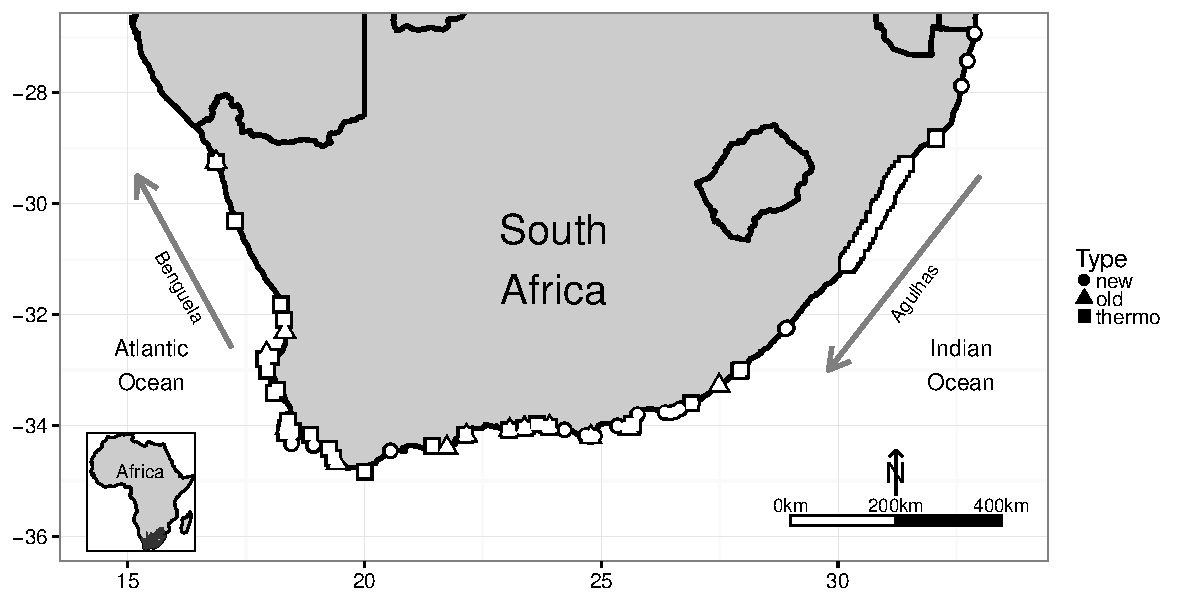
\includegraphics[width=1.0\textwidth]{figure01}
\caption[\small Location and instrument types used to sample each time series available for use in this study]{Location and instrument types used to sample each time series available for use in this study. In the legend, `new' shows the underwater temperature recorder (UTR) time series that were recorded entirely with the newer UTRs that have a high precision of \SI{0.001}{\degreeCelsius}, `old' refers to UTR time series that were recorded, at least in part, with older UTRs and have data with precisions lower than \SI{0.001}{\degreeCelsius}. The `thermo' label shows the location of the thermometer time series.}
\label{figure01}
\end{figure}

\emph{RWS - No longer showing coastal classification.}
% \begin{figure}
% \centering 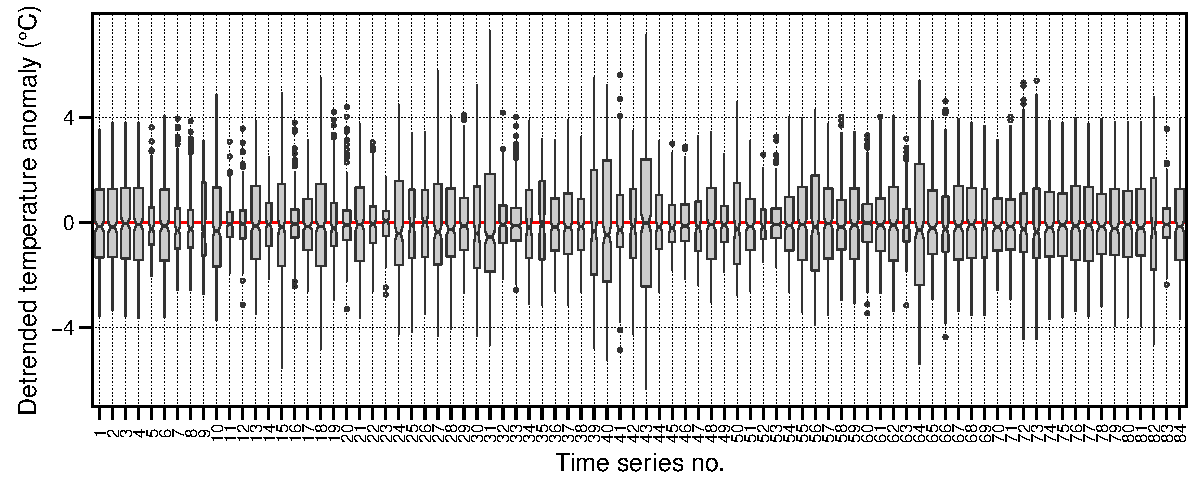
\includegraphics[width=1.0\textwidth]{figure02}
% \caption[\small Coastal allocation of time series from nonmetric multidimensional scaling and hierarchical cluster analysis]{Coastal allocation of time series from nonmetric multidimensional scaling and hierarchical cluster analysis.}
% \label{figure02}
% \end{figure}

\emph{RWS - No longer power analysis results. THis figure could be replaced by a box and whisker plot showing the normal distribution of the data.}
% \begin{figure}
% \centering 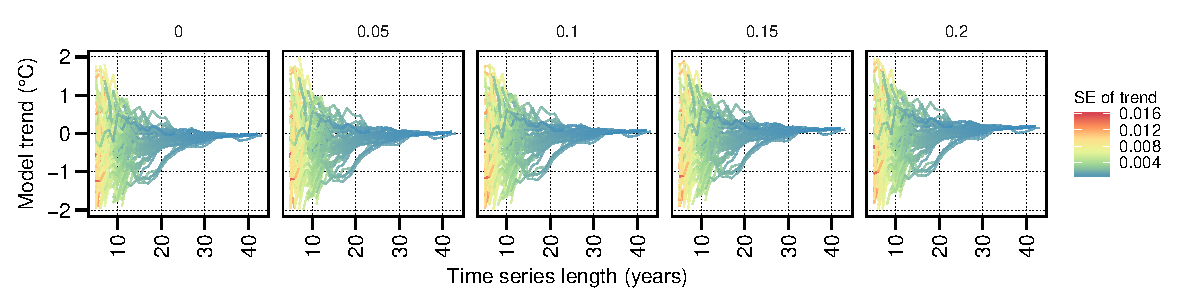
\includegraphics[width=0.66\textwidth]{figure03}
% \caption[\small Boxplots showing the range of lengths required for each subgroup to expect results from a time series analysis with a power of 0.80 or 0.90]{Boxplots showing the range of lengths required for each subgroup to expect results from a time series analysis with a power of 0.80 or 0.90. The median length required for each subgroup is denoted here with thick vertical bars. The ends of the boxplots show the 25th and 75th percentiles. The 95th percentile is shown as text to the left of each boxplot as they distort the range of the \emph{x}-axis. The \emph{n} values listed to the left of each subgroup shows how many time series were drawn on to calculate the statistics for the corresponding boxplots.}
% \label{figure03}
% \end{figure}

\emph{RWS - To be replaced with a new figure.}
% \begin{figure}
% \centering 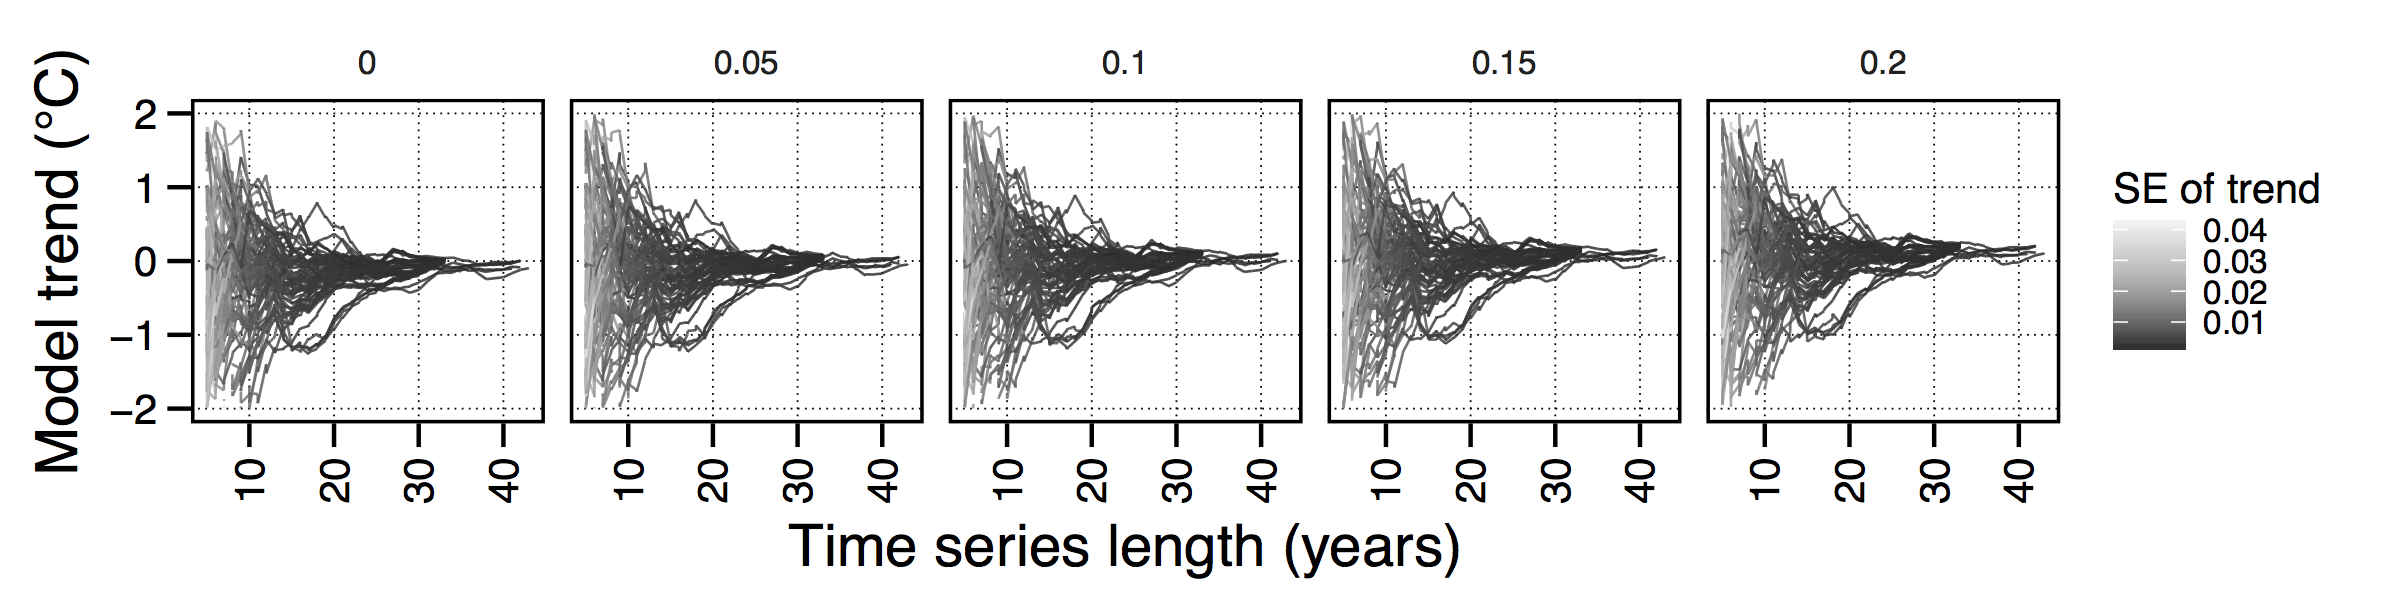
\includegraphics[width=0.66\textwidth]{figure04}
% \caption[\small The effect varying length has on the goodness of fit (\emph{R}\textsuperscript{2}) and significance (\emph{p}) of a linear model fitted to a time time series]{The effect varying length has on the goodness of fit (\emph{R}\textsuperscript{2}) and significance (\emph{p}) of a linear model fitted to a time time series. The number of time series available (\emph{n}) at length 36 months and then for every 60 month interval thereafter for each sub group shown in black in each panel. The median \emph{R}\textsuperscript{2} values are shown as series of dots whose shade shows the median \emph{p} value for that month. \emph{p} values less than 0.05 are shown as black dots, \emph{p} values under 0.10 as grey dots and \emph{p} values greater than 0.10 shown as white dots. The grey ribbon surrounding the dot plot shows the range (5th to 95th percentile) of the \emph{R}\textsuperscript{2} values from each time series for each new month.}
% \label{figure04}
% \end{figure}

\emph{RWS - To be replaced with a new figure.}
% \begin{figure}
% \centering 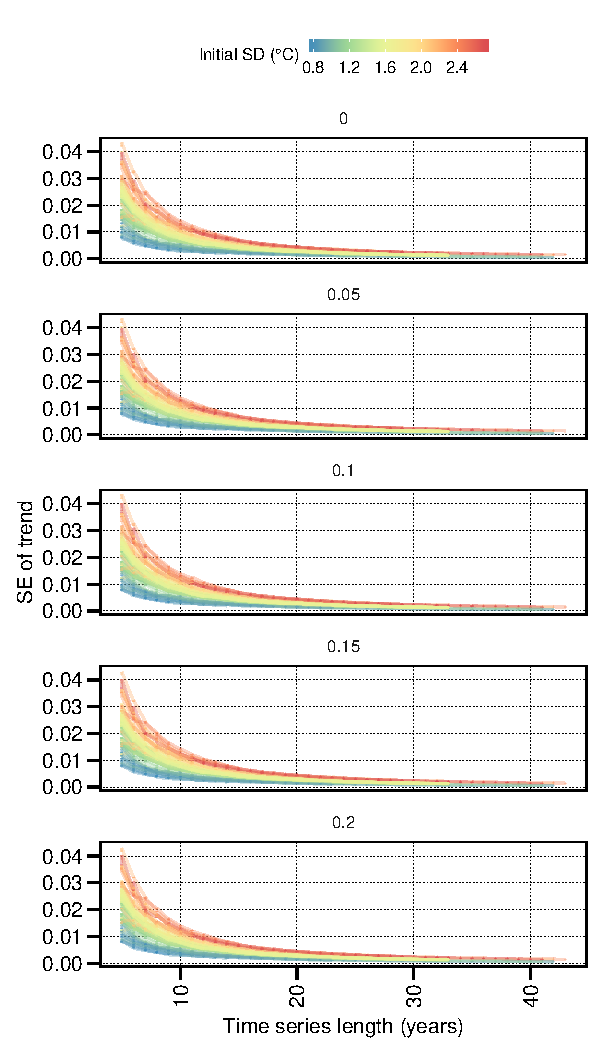
\includegraphics[width=0.66\textwidth]{figure05}
% \caption[\small The effect changes in the SD variable has on the goodness of fit (\emph{R}\textsuperscript{2}) and significance (\emph{p}) of a simple linear model fitted to a time series]{The effect changes in the SD variable has on the goodness of fit (\emph{R}\textsuperscript{2}) and significance (\emph{p}) of a simple linear model fitted to a time series. The number of time series (\emph{n}) used to calculate the effect of varying standard deviation (SD) for each subgroup shown in black in the top right of the corresponding panel. The dots show the median \emph{R}\textsuperscript{2} value for all time series within the corresponding subgroup with the given SD value as seen on the x-axis while the grey ribbon shows the 5th to 95th percentiles for the corresponding point. The colour of each point shows the median \emph{p} value with the same scale as Figure \ref{figure04}.}
% \label{figure05}
% \end{figure}

\end{document}
